\documentclass[ignorenonframetext,]{beamer}

\setbeamertemplate{caption}[numbered]
\setbeamertemplate{caption label separator}{: }
\setbeamercolor{caption name}{fg=normal text.fg}

\beamertemplatenavigationsymbolsempty
\usepackage{lmodern}
\usepackage{amssymb,amsmath}
\usepackage{ifxetex,ifluatex}
\usepackage{fixltx2e} % provides \textsubscript
\ifnum 0\ifxetex 1\fi\ifluatex 1\fi=0 % if pdftex
  \usepackage[T1]{fontenc}
  \usepackage[utf8]{inputenc}
\else % if luatex or xelatex
  \ifxetex
    \usepackage{mathspec}
  \else
    \usepackage{fontspec}
  \fi
  \defaultfontfeatures{Ligatures=TeX,Scale=MatchLowercase}
\fi

% Start adding some content
\usepackage{graphicx}
\usepackage{color}
\usepackage{beamerthemebars}
\usepackage{multicol}
\usepackage{multirow}
\usepackage{hyperref}


\usetheme{Frankfurt}
%%redefined colors for beamer
%\definecolor{beamer@UIUCblue}{RGB}{0,60,125}
%\definecolor{beamer@UIUCorange}{RGB}{244,127,36}
%% taken from
%% http://identitystandards.illinois.edu/graphicstandardsmanual/generalguidelines/colors.html
%
%\definecolor{beamer@UIUCgray}{RGB}{210,210,210}
%\definecolor{beamer@UIUCgray2}{RGB}{244,244,244}
%
%\setbeamercolor{frametitle}{fg=beamer@UIUCblue,bg=beamer@UIUCgray}
%\setbeamercolor{normal text}{fg=black}
%\setbeamercolor{title}{fg=beamer@UIUCblue,bg=beamer@UIUCorange}
%\setbeamercolor{item projected}{fg=white,bg=beamer@UIUCorange}
%
%% Boxes
%\setbeamercolor{block title}{fg=beamer@UIUCblue,bg=beamer@UIUCorange}
%\setbeamercolor{block body}{fg=blue,bg=beamer@UIUCblue!80}
%\setbeamercolor{title in head/foot}{fg=beamer@UIUCblue,bg=beamer@UIUCgray}
%\setbeamercolor{author in head/foot}{fg=white,bg=beamer@UIUCblue}
%\setbeamercolor{institute in head/foot}{fg=white,bg=beamer@UIUCorange}
%\setbeamercolor{date in head/foot}{fg=white,bg=beamer@UIUCorange}
%\setbeamercolor{section in head/foot}{fg=white,bg=beamer@UIUCblue}
%\setbeamercolor{subsection in head/foot}{fg=white,bg=beamer@UIUCorange}
%
%
%\hypersetup{colorlinks=true,urlcolor=beamer@UIUCblue,linkcolor=beamer@UIUCblue,% link color controls section, subsection, and title
%citecolor = beamer@UIUCorange,
%anchorcolor = beamer@UIUCorange}
%
%%override title link color
%\addtobeamertemplate{headline}{\hypersetup{linkcolor=.}}{}
%\addtobeamertemplate{footline}{\hypersetup{linkcolor=.}}{}
%
%% Setup blocks
%\setbeamercolor{block title}{fg = white, bg = beamer@UIUCblue}
%\setbeamercolor{block body}{fg=black,bg=beamer@UIUCgray2}
%
%\setbeamercolor{block title alerted}{fg = white, bg = beamer@UIUCorange}
%\setbeamercolor{block body alerted}{fg=black,bg=beamer@UIUCgray2}
%
%\setbeamercolor{block title example}{fg = beamer@UIUCblue, bg = beamer@UIUCgray}
%\setbeamercolor{block body example}{fg=black,bg=beamer@UIUCgray2}

% use upquote if available, for straight quotes in verbatim environments
\IfFileExists{upquote.sty}{\usepackage{upquote}}{}
% use microtype if available
\IfFileExists{microtype.sty}{%
\usepackage{microtype}
\UseMicrotypeSet[protrusion]{basicmath} % disable protrusion for tt fonts
}{}
\newif\ifbibliography
\usepackage{graphicx,grffile}
\makeatletter
\def\maxwidth{\ifdim\Gin@nat@width>\linewidth\linewidth\else\Gin@nat@width\fi}
\def\maxheight{\ifdim\Gin@nat@height>\textheight0.8\textheight\else\Gin@nat@height\fi}
\makeatother
% Scale images if necessary, so that they will not overflow the page
% margins by default, and it is still possible to overwrite the defaults
% using explicit options in \includegraphics[width, height, ...]{}
\setkeys{Gin}{width=\maxwidth,height=\maxheight,keepaspectratio}

% Prevent slide breaks in the middle of a paragraph:
\widowpenalties 1 10000
\raggedbottom

\AtBeginSection[]
{
  \ifbibliography
  \else
    \let\insertsectionnumber\relax
    \let\sectionname\relax
    \begin{frame}
      \frametitle{On the Agenda}
      \begin{multicols}{2}
      \tableofcontents[currentsection]
      \end{multicols}
    \end{frame}
  \fi
}

\setlength{\parindent}{0pt}
\setlength{\parskip}{6pt plus 2pt minus 1pt}
\setlength{\emergencystretch}{3em}  % prevent overfull lines
\providecommand{\tightlist}{%
  \setlength{\itemsep}{0pt}\setlength{\parskip}{0pt}}
\setcounter{secnumdepth}{0}
\usepackage{amsmath, bbm, graphicx,multirow}
\usepackage{booktabs}
\usepackage{longtable}
\usepackage{array}
\usepackage{multirow}
\usepackage{wrapfig}
\usepackage{float}
\usepackage{colortbl}
\usepackage{pdflscape}
\usepackage{tabu}
\usepackage{threeparttable}
\usepackage{threeparttablex}
\usepackage[normalem]{ulem}
\usepackage{makecell}
\usepackage{xcolor}
\newcommand{\indep}{\rotatebox[origin=c]{90}{$\models$}}


\author[
Xuelong Wang and Jie Yang
]{Xuelong Wang and Jie Yang}
\institute[
UIC
]{
Department of Mathematics, Computer Science, and Statistics \\
University of Illinois at Chicago
}
\date[
09/04/2019
]{
September 04, 2019
}

% Option to fake out the raw_tex plugin and, thus, enabling the embedding of
% markdown within a column scheme.
% See:
% (1) https://groups.google.com/forum/#!msg/pandoc-discuss/vcy7v9Uk95U/LDgWJTHTRR4J
% (2) http://stackoverflow.com/questions/15142134/slides-with-columns-in-pandoc
\def\begincols{\begin{columns}}
\def\endcols{\end{columns}}

\begin{document}

% Necessary due to the ignorenonframetext requirement
% See: http://tex.stackexchange.com/questions/181032/ignorenonframetext-option-breaks-frame-background-color-option
\mode<all>{
\title[
Representative approach
]{
%\begin{columns}
%\column{.25\textwidth}
%\hspace{.2in}
%\vspace{.1in}
%\includegraphics{ilogo.pdf}
%\column{.85\textwidth}
Representative approach for big data dimension reduction with binary
responses
%\end{columns}
}
}
\mode*

\frame{\titlepage}

\begin{frame}
\tableofcontents[hideallsubsections]
\end{frame}

\section{Background}\label{background}

\subsection{Motivation}\label{motivation}

\begin{frame}{Motivation of reducing the dimension of the data}

\begin{block}{Curse of dimensionality (p is large)}

\begin{itemize}
\tightlist
\item
  Data becomes sparse (need more data to get same level of accuracy)
\item
  Model Overfitting
\end{itemize}

\end{block}

\begin{block}{Two approaches}

\begin{enumerate}
\def\labelenumi{\arabic{enumi}.}
\tightlist
\item
  Variable selection (feature selection)

  \begin{itemize}
  \tightlist
  \item
    Forward/Backward selection, Lasso, etc.
  \end{itemize}
\item
  \textbf{Dimension reduction} (feature projection)

  \begin{itemize}
  \tightlist
  \item
    Principle component analysis
  \item
    Sufficient dimension reduction
  \end{itemize}
\end{enumerate}

\end{block}

\end{frame}

\begin{frame}{An example: Breast Cancer data}

\begin{block}{Data}

Features are computed from a digitized image of a fine needle aspirate
(FNA) of a breast mass

\begin{itemize}
\tightlist
\item
  Y: Diagnosis results (1 = malignant, 0 = benign)
\item
  X: 30 features of each each cell nucleus

  \begin{itemize}
  \tightlist
  \item
    e.g.~radius, texture, area
  \end{itemize}
\end{itemize}

picture

\end{block}

\begin{block}{Goal}

Classificantion: Diagnose breast cancer from image-processed nuclear
features of fine needle aspirates

\end{block}

\end{frame}

\begin{frame}{An example: Breast Cancer data}

\begin{center}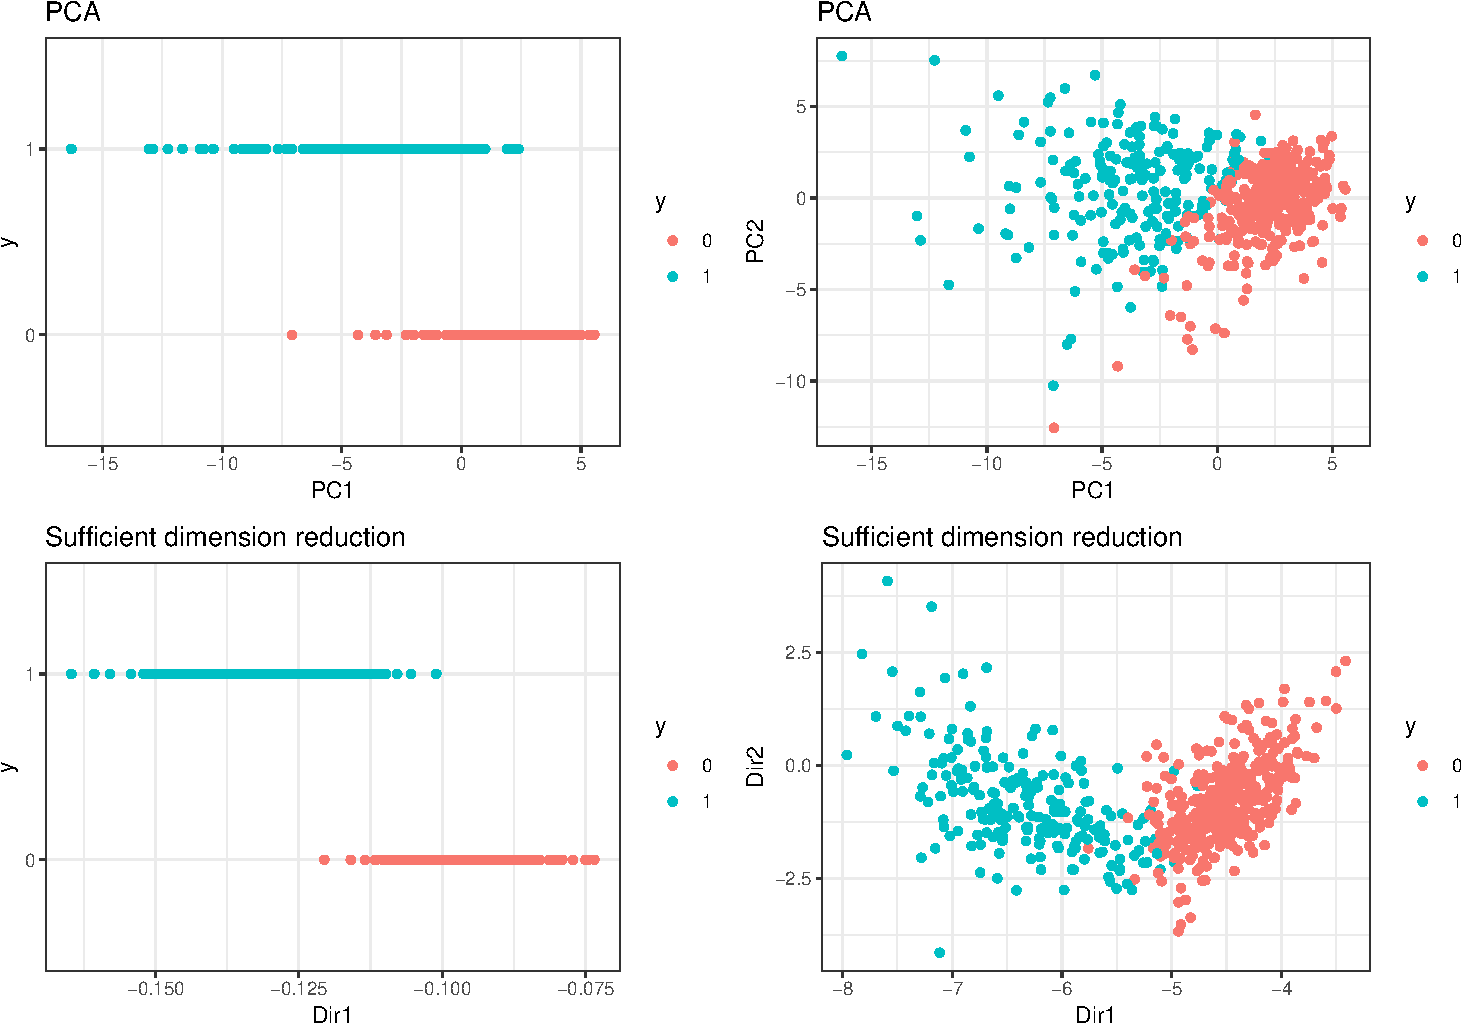
\includegraphics{SDR_reps_slides_final_merck_files/figure-beamer/unnamed-chunk-2-1} \end{center}

\end{frame}

\subsection{SDR}\label{sdr}

\begin{frame}{Subspace}

\begin{itemize}
\item
  Vector space U: \(\vec{\mathbf{a}}, \vec{\mathbf{b}} \in U\)

  \begin{enumerate}
  \def\labelenumi{\arabic{enumi}.}
  \tightlist
  \item
    \(\vec{\mathbf{a}} + \vec{\mathbf{b}} \in U\)\\
  \item
    \(\lambda \vec{\mathbf{a}} \in U, \lambda \in \mathbb{R}\)
  \end{enumerate}
\item
  Subspace \(V\): Given k independent vectors
  \((\vec{\mathbf{a}}_1, \dots, \vec{\mathbf{a}}_k), ~~\vec{\mathbf{a}}_i \in \mathbb{R}^p\),
  \[
  V = \mathcal{L}((\vec{\mathbf{a}}_1, \dots, \vec{\mathbf{a}}_k) = \{\sum_{i = 1}^k\lambda_ia_i, \lambda_i\in \mathbb{R}\}
  \] \(V\) is spaced by
  \((\vec{\mathbf{a}}_1, \dots, \vec{\mathbf{a}}_k)\)
\item
  A basis of \(V\): \((\vec{\mathbf{a}}_1, \dots, \vec{\mathbf{a}}_k)\)
  is called a basis of \(V\), but it is not unique
\end{itemize}

\end{frame}

\begin{frame}{Sufficient dimension reduction}

\begin{block}{Fundamental assumption}

Let random vector \(X \in \mathbb{R}^{p \times 1}\),
\(Y \in \mathbb{R}\),
\(B = (b_1, \dots,b_d) \in \mathbb{R}^{p\times d}\), where \(d << p\)
and \(A \in \mathbb{R}^{d\times d}\) is a non-singular matrix. \[
Y|X \stackrel{d}{=} Y|B^T X
\]

\[
  Y \indep X|B^TX \Rightarrow Y \indep X|(BA)^TX, 
\] So \(B\) is not identifiable, but \(span(B)\) is identifiable.

\end{block}

\end{frame}

\begin{frame}{Sufficient dimension reduction}

\begin{block}{Dimension-reduction subspace (DRS)}

\[
  Y \indep X|P_SX,~~ P_\mathcal{S} = B(B^TB)^{-1}B^T
\] \(\mathcal{S}\) is called the dimension-reduction subspace.

However,\(\mathcal{S}\) is not unique. Actually if
\(\mathcal{S} \subset \mathcal{S}_1\), then \(\mathcal{S}_1\) is also a
dimension-reduction space.

\end{block}

\begin{block}{Target: Central Subspace}

\[
S_{Y|X} = \cap S_{DRS}
\] Under mild conditions, \(S_{Y|X}\) is unique and a DRS subspace
itself (Cook, 1996).

\end{block}

\end{frame}

\begin{frame}{Comment}

\begin{itemize}
\tightlist
\item
  No model assumption between X and Y
\item
  Target is a subspace not a specific values coefficients
\end{itemize}

\end{frame}

\subsection{Estimating the central
subspace}\label{estimating-the-central-subspace}

\begin{frame}{Estimating the central subspace}

\begin{block}{Sliced Inverse Regression (SIR) (Li 1991)}
\[
E(X|Y) - E(X) \in \Sigma_XS_{Y|X} = Span(\Sigma_{X}b_i),i = 1, \dots, d
\]
\end{block}

\begin{enumerate}
\def\labelenumi{\arabic{enumi}.}
\tightlist
\item
  \(E(X|Y) - E(X)\) is p-dimensional curves as Y varies and lies in a
  k-dimensional subspace
\item
  The covariance matrix of \(E(X|Y) - E(X)\) is degenerate at any
  direction that orthogonal to \(\Sigma_{X}b_i,i = 1, \dots, d\)
\item
  Condidate Matrix: \(M_{SIR} = Var(E(X|Y) - E(X)) = Var(E(X|Y))\)
\item
  \(S_{SIR} := Span(\Sigma_{X}^{-1}M_{SIR}) \subseteq S_{Y|X}\)
\item
  \(\Sigma_{X}^{-1}M_{SIR}b_i = \lambda_i b_i\) \(b_i\) is the ith
  eigenvector of \(\Sigma_{X}^{-1}M_{SIR}\)
\end{enumerate}

\end{frame}

\begin{frame}{Estimating the central subspace (cont.)}

\begin{block}{Sliced Average Variance Estimation (SAVE) (Cook et al. 1991)} 
\[
span(\Sigma_x - \Sigma_{X|\tilde{Y}}) \subseteq S_{Y|X} \Rightarrow  ({b}_1, \dots, {b}_d)
\]
\end{block}

\begin{itemize}
\tightlist
\item
  There are many other methods using first and second monments togehter

  \begin{itemize}
  \tightlist
  \item
    Directional regression etc.
  \end{itemize}
\end{itemize}

\end{frame}

\begin{frame}{How to estimate the \(E(X|Y)\), \(\Sigma_{X|\tilde{Y}}\)?}

\begin{enumerate}
\def\labelenumi{\arabic{enumi}.}
\tightlist
\item
  Sort the data based on the response \[
    Y_1 \dots, Y_n \Rightarrow Y^{(1)},\dots,Y^{(n)} 
  \]
\item
  Split data into H slices and set \(Y = \tilde{Y}_h, h = 1,\dots H\)
\item
  Within the slice h, calculate the average of X,
  \[\tilde{X}_h = \hat{E}(X|Y = \tilde{Y}_h)\]
  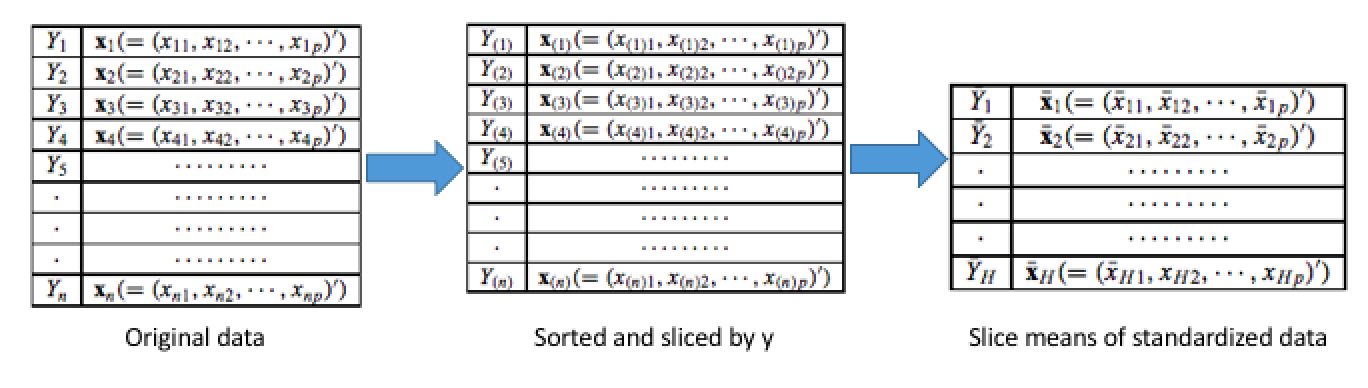
\includegraphics[width=4.16667in]{./pic/slice method.png}
\end{enumerate}

\end{frame}

\begin{frame}{Issue with Binary response}

\begin{itemize}
\item
  Binary response only has two levels, e.g. \(0,1\).
\item
  Only two slices are available after slicing
\item
  SIR can only find one direction
\end{itemize}

\end{frame}

\section{Existing solution}\label{existing-solution}

\subsection{Variance matrix}\label{variance-matrix}

\begin{frame}{Using conditional variance (Cook. 1999)}

\begin{block}{Main Idea}

\(\Delta = \Sigma_{X|Y = 1} - \Sigma_{X|Y = 0}\) could contain all the
information of the central space

\end{block}

\begin{block}{Not full rank}

There is cases that \(\hat \Delta\) is not full rank or even is 0 matrix

\end{block}

\end{frame}

\subsection{PRE}\label{pre}

\begin{frame}{Probability Enhanced (PRE) method (Shin et al. 2014)}

\begin{block}{Main idea}

\begin{itemize}
\tightlist
\item
  \(S_{Y|X} = S_{G(X)}\), \(G(x) = \mathcal{P}(Y = 1|X = x)\) is the
  conditional probability
\item
  \(Y \Rightarrow G(X) \in [0,1]\)
\item
  Weighted Support Vector Machine(WSVM) to estimate the \(\hat{G}(X)\)
\end{itemize}

\end{block}

\begin{block}{Computational time}

\begin{itemize}
\tightlist
\item
  SVM method is sensitive to the number of observation N
\item
  Tunning parameters
\end{itemize}

\end{block}

\end{frame}

\section{Our approach}\label{our-approach}

\subsection{Rep}\label{rep}

\begin{frame}{Representative approach}

\begin{block}{Representative}

A Representative is a summary statistic of data points within a cluster:
For \((X_i, Y_i), i \in I_k\) and \(n_k\) is sample size of \(I_k\) \[
  \bar{X}_k = R(X_{1}, \dots, X_{n_k}) = \frac{\sum_i X_i}{n_k},~~ \bar{Y}_k = R(Y_{1}, \dots, Y_{n_k}) = \frac{\sum_i Y_i}{n_k},
\] where \(R\) is the summarizing function.

\end{block}

\begin{block}{Steps}

\begin{enumerate}
\def\labelenumi{\arabic{enumi}.}
\tightlist
\item
  Cluster \((X_1, \dots,X_N)\) into k groups \(I_1, \dots, I_k\),
  e.g.k-means
\item
  Calculate the representatives for each cluster \(I_k\)
\item
  Apply dimension reduction methods on the k representatives
\end{enumerate}

\end{block}

\end{frame}

\begin{frame}{How it works}

\begin{block}{Main idea}

Y and \(G(X)\) have identical central space: \(S_{Y|X} = S_{G(X)|X}\)

\begin{center}
$Y = f(b_1^TX, \dots, b_d^TX,\epsilon)$
$\Rightarrow$
$\mathcal{P}(Y = 1 |X) = G(b_1^TX, \dots, b_d^TX)$
\end{center}

\end{block}

\begin{block}{For the Representative}

\begin{center}
$\bar{Y}_k = \hat{\mathcal{P}}(Y = 1|X_i, i\in I_k) \approx G(b_1^T\bar{X}_k, \dots, b_d^T\bar{X}_k)$
\end{center}

\end{block}

\end{frame}

\begin{frame}{Aysmptotic property with fixed clusters}

\begin{block}{Fixed cluster}
\begin{align*}
\bar{Y}_k - G(\bar{\mathbf X}_k) &\stackrel{P}{\longrightarrow} \mu_g - G(\boldsymbol{\mu}_k)\\
& = p_k^{-1} \int_{B_k} G({\mathbf x}) F(d{\mathbf x}) - G\left(p_k^{-1} \int_{B_k} {\mathbf x} F(d{\mathbf x})\right)
\end{align*}
\end{block}

\begin{itemize}
\tightlist
\item
  Note that with fixed cluster, there is a bias between the
  representative version of conditional probability
\item
  To remove the bias we need to reduce the size of cluster when N is
  increaseing
\end{itemize}

\end{frame}

\begin{frame}{Aysmptotic property with shrinking clusters}

\begin{block}{Shrinking cluster}
\[
E([\bar{Y}_k - G(\bar{\mathbf X}_k)]^2) = O(N^{-\delta(r)})
\]
\end{block}

Where \(\delta(r) = \min\{4/(rd), 1-1/r\}\) for \(r>1\), which is
maximized at \(r = 1 + 4/d\). In other words, the minimum decreasing
rate of \(E([\bar{Y}_k - G(\bar{\mathbf X}_k)]^2)\) is
\(O(N^{-4/(d+4)})\) which is attained at \(r= 1 + 4/d\).

\end{frame}

\begin{frame}{Additional value: Big data solution (N is large)}

\begin{block}{Clustering step}

Clustering step reduced the sample size from \(N\) to \(k\).

\begin{itemize}
\item
  \((Y_1,X_1) \dots (Y_N,X_N) \to (Y^*_{1},X^*_{1}) \dots (\bar{Y}_k,\bar{X}_k)\)
\item
  Note if the data set is too large, we could also use the online
  clustering method.
\end{itemize}

\end{block}

\end{frame}

\begin{frame}{Additional value: Big data solution (N is large)}

\begin{block}{Parallel Algorithm for SIR and SAVE}

\begin{enumerate}
\def\labelenumi{\arabic{enumi}.}
\tightlist
\item
  Split the sliced data into b blocks, \(X_1, \dots X_B\)\\
\item
  Load each block \(X_b\) and calculate the statistics for each block
  such as \(\bar{X}_b, \bar{X}_{hb}, n_{hb}, X^T_{hb}X_{hb}\)\\
\item
  Summary the statistics across the blocks and slices to get the
  candidate matrix \(M_{SIR}, M_{SAVE}\)
\end{enumerate}

\end{block}

\end{frame}

\section{Simulation Study}\label{simulation-study}

\subsection{}\label{section}

\begin{frame}{Simulation setup}

\begin{block}{Data generation model: logit model}
\[
    \log\left(\frac{\mathcal{P}(Y=1|X=x)}{1-\mathcal{P}(Y=1|X=x)}\right) = b_1^Tx \cdot sin(b_2^Tx) \cdot exp(b_3^Tx)
\]

- $n = \{10^3, 10^4, 10^5,10^6\}$  
- $X \in \mathbb{R}^6$  
- $b_1 = e_i = (0, \dots, 1, \dots,0) \in \mathbb{R}^6$  
- $S_{Y|X} = Span(e_1, e_2, e_3)$  
\end{block}

Note that the central subspace is a 3-dimensional subspace in a
6-dimensional space

\end{frame}

\begin{frame}{How to evaluate esimated central subspace}

\begin{block}{The number of direction}

\begin{enumerate}
\def\labelenumi{\arabic{enumi}.}
\tightlist
\item
  Hypothesis Test: test if a eigenvalue is significant than 0
\item
  Ad-hoc: select all the eigenvalues whcih are larger then a cutoff
  value
\end{enumerate}

\end{block}

\begin{block}{The distrance of the true subspace}

\begin{enumerate}
\def\labelenumi{\arabic{enumi}.}
\tightlist
\item
  Fourbin distance
\item
  trace correlation
\end{enumerate}

\end{block}

\end{frame}

\begin{frame}{Simulation result of SAVE}

\begin{table}[]
\centering
\caption{Simulation result of SAVE}
\resizebox{\textwidth}{!}{%
\begin{tabular}{|c|c|cccc|cccc|}
\hline
\multicolumn{2}{|c|}{\multirow{2}{*}{}}              & \multicolumn{4}{c|}{Original SAVE} & \multicolumn{4}{c|}{Proposed SAVE}                \\ \cline{3-10} 
\multicolumn{2}{|c|}{}                               & \multicolumn{8}{c|}{log n}                                                      \\ \hline
                          & $H_0$ vs $H_1$       & 3      & 4      & 5      & 6      & 3    & 4    & 5             & 6             \\ \hline
\multirow{3}{*}{Power}    & 0D vs \textgreater{}= 1D & 0.9    & 1      & 1      & 1      & 0    & 0.05 & \color{blue}\textbf{1}    & \color{blue}\textbf{1}    \\
                          & 1D vs \textgreater{}= 2D & 0.08   & 0.52   & 0.52   & 0.5    & 0    & 0    & \color{blue}\textbf{1}    & \color{blue}\textbf{1}    \\
                          & 2D vs \textgreater{}= 3D & 0      & 0.05   & 0.06   & 0.06   & 0    & 0    & 0.05          & \color{blue}\textbf{1}    \\ \hline
\multirow{3}{*}{Type-I}   & 3D vs \textgreater{}= 4D & 0      & 0      & 0      & 0.01   & 0    & 0    & 0             & 0.14          \\
                          & 4D vs \textgreater{}= 5D & 0      & 0      & 0      & 0      & 0    & 0    & 0             & 0.03             \\
                          & 5D vs \textgreater{}= 6D & 0      & 0      & 0      & 0      & 0    & 0    & 0             & 0.02             \\ \hline
\multirow{2}{*}{Distance} & F                        & 1.47   & 1.2    & 1.21   & 1.21   & . & 1.44 & \color{blue}\textbf{1.00} & \color{blue}\textbf{0.39} \\
                          & R                        & 0.06   & 0.01   & 0.01   & 0.01   & . & 0.02  & \color{blue}\textbf{0.01} & \color{blue}\textbf{0.04}    \\ \hline
\end{tabular}%
}
\end{table}

\end{frame}

\begin{frame}{Simulation result of SIR}

\begin{table}[]
\centering
\caption{Simulation result of SIR}
\resizebox{\textwidth}{!}{%
\begin{tabular}{|c|c|cccc|cccc|cccc|}
\hline
\multicolumn{2}{|l|}{\multirow{2}{*}{}}              & \multicolumn{4}{c|}{SIR\_Binary} & \multicolumn{4}{c|}{SIR\_PRE} & \multicolumn{4}{c|}{SIR\_R}                 \\ \cline{3-14}
\multicolumn{2}{|l|}{}                               & \multicolumn{12}{c|}{log n}                                                                                    \\ \hline
\multicolumn{1}{|l|}{}    & Direction/Distance       & 3      & 4      & 5      & 6     & 3        & 4    & 5    & 6    & 3    & 4          & 5          & 6          \\
\multirow{3}{*}{Power}    & 0D vs \textgreater{}= 1D & 1      & 1      & 1      & 1     & 1        & .    & .    & .    & 0.75 & \color{blue}\textbf{1} & \color{blue}\textbf{1} & \color{blue}\textbf{1} \\
                          & 1D vs \textgreater{}= 2D & .      & .      & .      & .     & 1        & .    & .    & .    & 0.16 & \color{blue}\textbf{1} & \color{blue}\textbf{1} & \color{blue}\textbf{1} \\
                          & 2D vs \textgreater{}= 3D & .      & .      & .      & .     & 1     & .    & .    & .    & 0.01 & 0.01       & 0          & 0.01       \\ \hline
\multirow{3}{*}{Type-I}   & 3D vs \textgreater{}= 4D & .      & .      & .      & .     & 0      & .    & .    & .    & 0    & 0          & 0          & 0          \\
                          & 4D vs \textgreater{}= 5D & .      & .      & .      & .     & 0      & .    & .    & .    & 0    & 0          & 0          & 0          \\
                          & 5D vs \textgreater{}= 6D & .      & .      & .      & .     & 0    & .    & .    & .    & 0    & 0          & 0          & 0          \\ \hline
\multirow{2}{*}{Distance} & F                        & 1.14   & 1.12   & 1.14   & 1.13  & \color{red}\textbf{0.88}     & .    & .    & .    & 1.47 & 1.13       & \color{blue}\textbf{1.01}       & \color{blue}\textbf{1}       \\
                          & R                        & 0.01   & 0   & 0   & 0  & \color{blue}\textbf{0.06}     & .    & .    & .    & 0.06 & \color{blue}\textbf{0.02}   & \color{blue}\textbf{0}       & \color{blue}\textbf{0}       \\ \hline
\end{tabular}%
}
\end{table}

\end{frame}

\section{Conclusion}\label{conclusion}

\begin{frame}{Conclusion and Future work}

\begin{block}{Conclusion}

\begin{itemize}
\tightlist
\item
  Better recover the central space in binary responses
\item
  Greatly shorten the running time in big data
\end{itemize}

\end{block}

\begin{block}{Future work}

\begin{itemize}
\tightlist
\item
  Investigate optimal the choice of k to achieve the best performance of
  SDR methods.
\end{itemize}

\end{block}

\end{frame}

\begin{frame}{Reference}

\hypertarget{refs}{}
\hypertarget{ref-ref7}{}
Cook, R Dennis, and Sanford Weisberg. 1991. ``Discussion of `Sliced
Inverse Regression for Dimension Reduction'.''

\hypertarget{ref-ref9}{}
Kim, Boyoung, and Seung Jun Shin. 2019. ``Principal Weighted Logistic
Regression for Sufficient Dimension Reduction in Binary
Classification.''

\hypertarget{ref-ref6}{}
Li, Ker-Chau. 1991. ``Sliced Inverse Regression for Dimension
Reduction.''

\hypertarget{ref-ref8}{}
Shin, Seung Jun, Yichao Wu, Hao Helen Zhang, and Yufeng Liu. 2014.
``Probability-Enhanced Sufficient Dimension Reduction for Binary
Classification.''

\end{frame}

\begin{frame}{Backup}

\begin{examples}

1. Linear regression: $Y = a + b_1^TX + b_2^TX + \epsilon$

2. NonLinear regression: $Y = a + \exp(b_1^TX) + \sin(b_2^TX) + \epsilon$

3. More general: $Y = f(b_1^TX, b_2^TX, \epsilon)$
\end{examples}

\end{frame}

\begin{frame}{SUSY data}

\end{frame}

\begin{frame}{SUSY data cont.}

\end{frame}

\end{document}
